\chapter*{Appendix}
\addcontentsline{toc}{chapter}{Appendix}

    \section*{List of Decorators}
    \label{app:decorators}
        This presents a non-exhaustive list of proposed \textbf{Decorators} types, as suggested by Alex J. Champandard~\cite{btdecorators}.
        \begin{itemize}
        \item \textbf{Filters}: These prevent a behavior from activating under certain circumstances.
            \begin{itemize}
                \item Limit the number of times a behavior can be run
                \item Prevent a behavior from firing too often with a timer
                \item Temporarily deactivate a behavior by script
                \item Restrict the number of behaviors running simultaneously
            \end{itemize}
        \item \textbf{Managers \& Handlers}: These are decorators that are responsible for managing whole subtrees rather than single behaviors. 
            \begin{itemize}
                \item Deal with the error status code and restart planning or execution
                \item Store information for multiple child nodes to access as a blackboard            
            \end{itemize}
        \item \textbf{Control Modifiers}: These decorators are used to pretend that the execution of the child node happened differently
            \begin{itemize}
                \item Force a return status, e.g. always fail or always succeed
                \item Fake a certain behavior, i.e. keep running instead of failing or succeeding   
            \end{itemize}
        \item \textbf{Meta Operations}: Such decorators are useful during development, and can be inserted into a tree automatically when needed.
            \begin{itemize}
                \item Debug breakpoint; pause execution and prompt the user
                \item Logging; track this node execution and print to the console
            \end{itemize}        
        \end{itemize}
        
    \newpage
        
    \section*{Project Backlog}
    \label{app:backlog}
        \begin{figure}        
        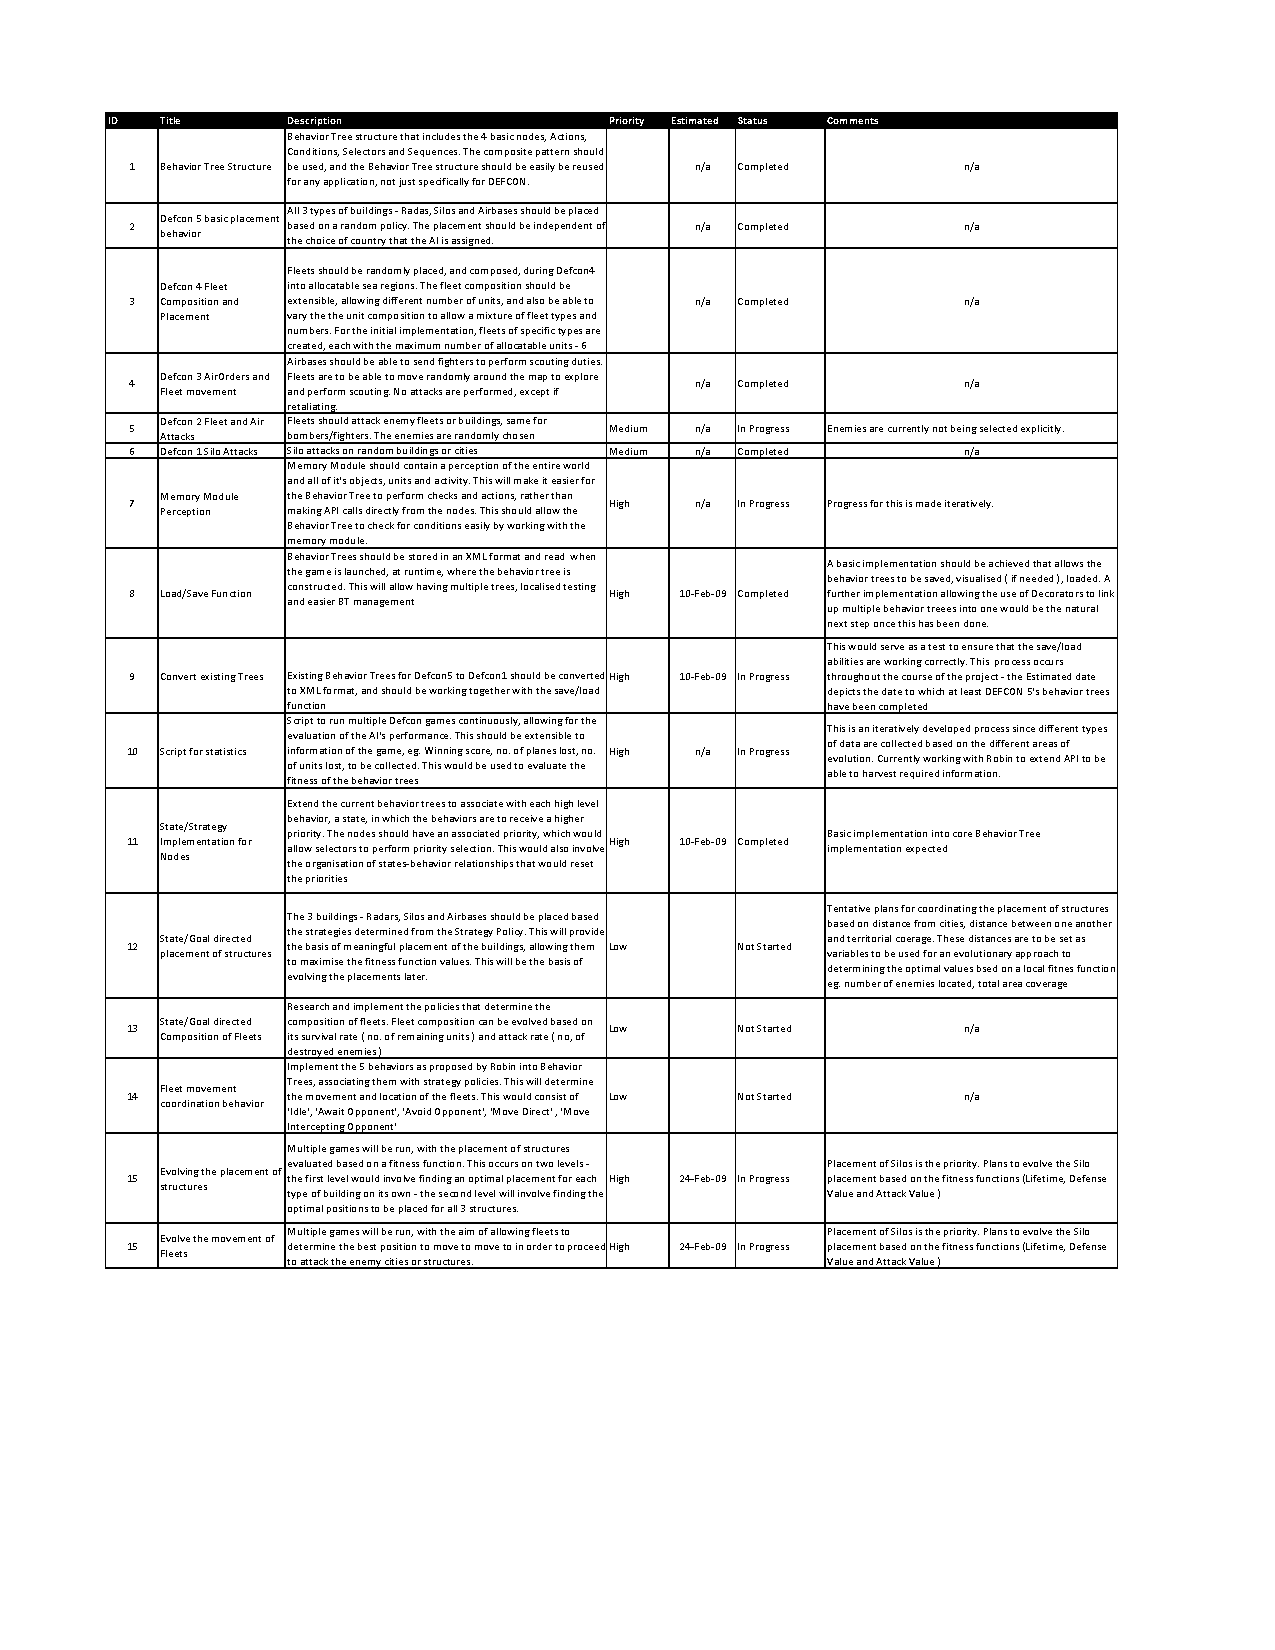
\includegraphics[bb=1.5in 2.0in 7.5in 9in,page=1]{backlog}
        \end{figure}
        
    \newpage
        
    \section*{DEFCON Behavior Trees}
    \label{app:defconbts}
    The tree diagrams here were automatically generated from the code. The nodes do not take the shape of the convention used in the report, instead nodes are prefixed to indicate the node types. The prefixes are:
    \begin{itemize}
    \item \textbf{ACT}: \texttt{Action} node
    \item \textbf{CON}: \texttt{Condition} node
    \item \textbf{SEL}: \texttt{Selector} node
    \item \textbf{SEQ}: \texttt{Sequence} node
    \item \textbf{PSEL}: \texttt{Priority Selector} node
    \end{itemize}
       
    \begin{figure}[h]
        \begin{center}
        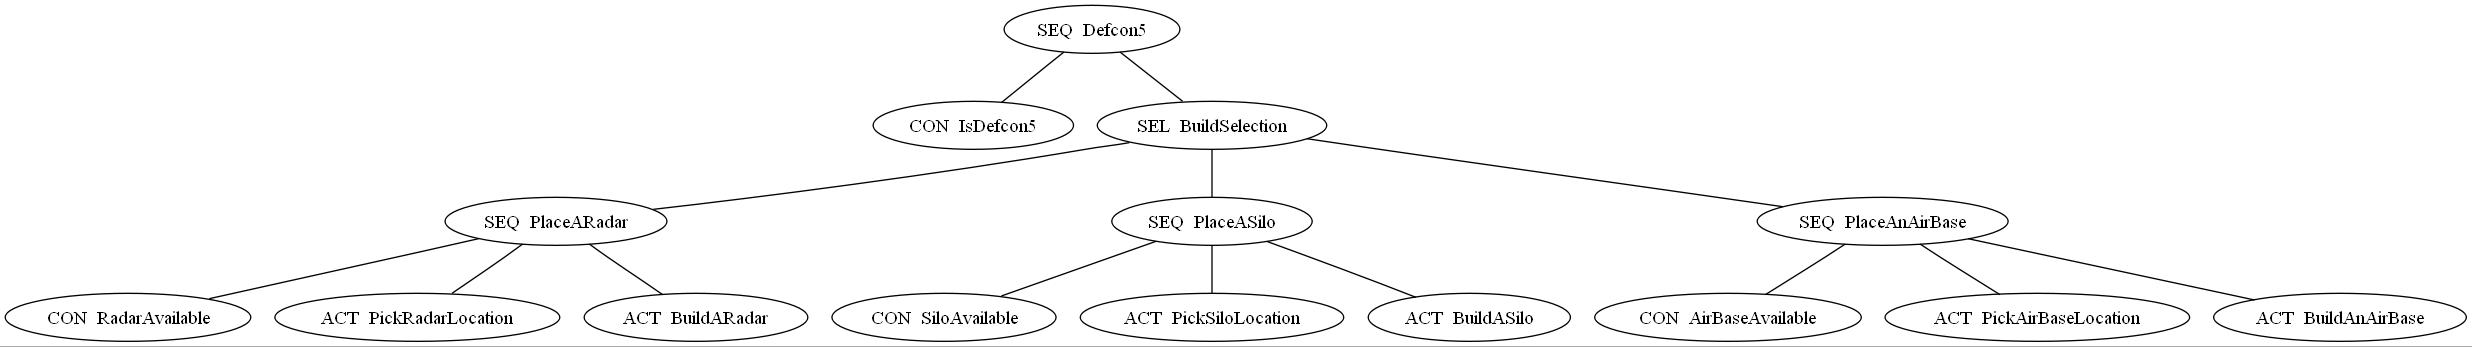
\includegraphics[scale=0.2, angle=270]{images/defcon5r.png}
        \caption{Defcon 5}        
        \end{center} 
    \end{figure}
    
    \begin{figure}[h]
        \begin{center}
        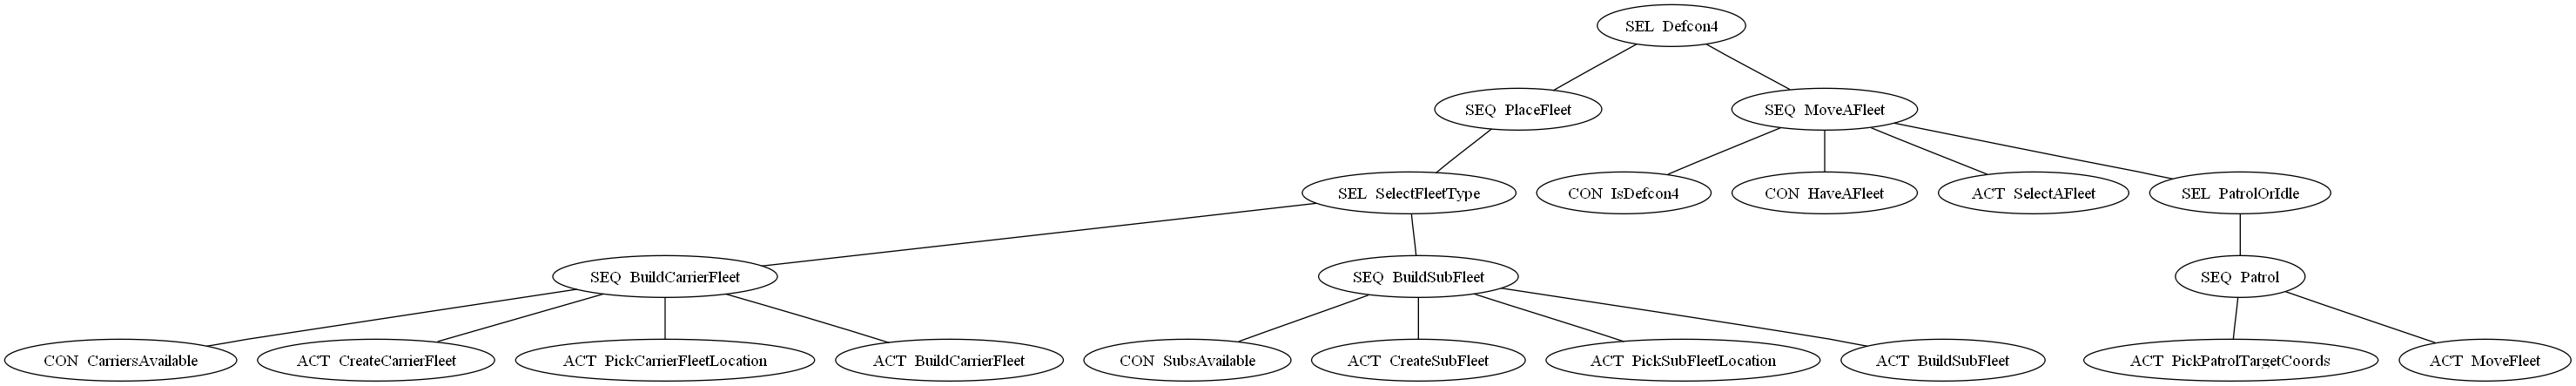
\includegraphics[scale=0.2, angle=270]{images/defcon4r.png}
        \caption{Defcon 4}  
        \label{app:d4}
        \end{center} 
    \end{figure}
    
    \begin{figure}[h]
        \begin{center}
        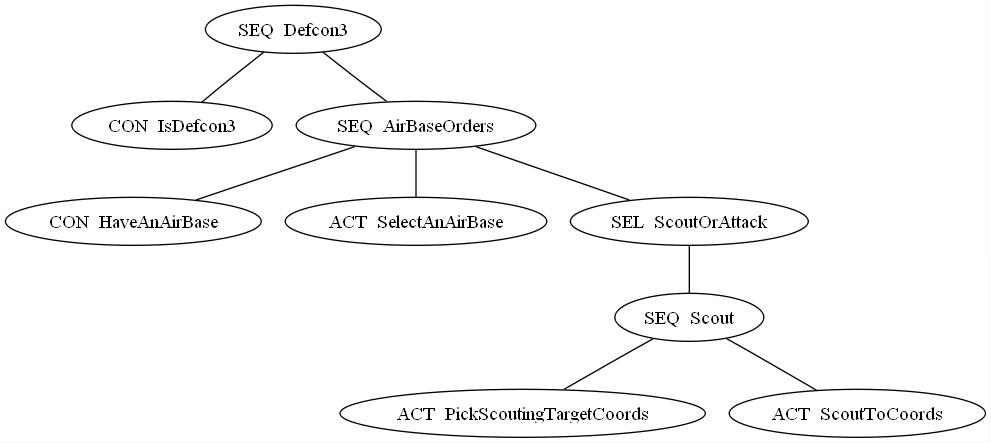
\includegraphics[scale=0.4]{images/defcon3r.png}
        \caption{ Defcon 3 and Defcon 2} 
        \end{center} 
    \end{figure}
    
    \begin{figure}[h]
        \begin{center}
        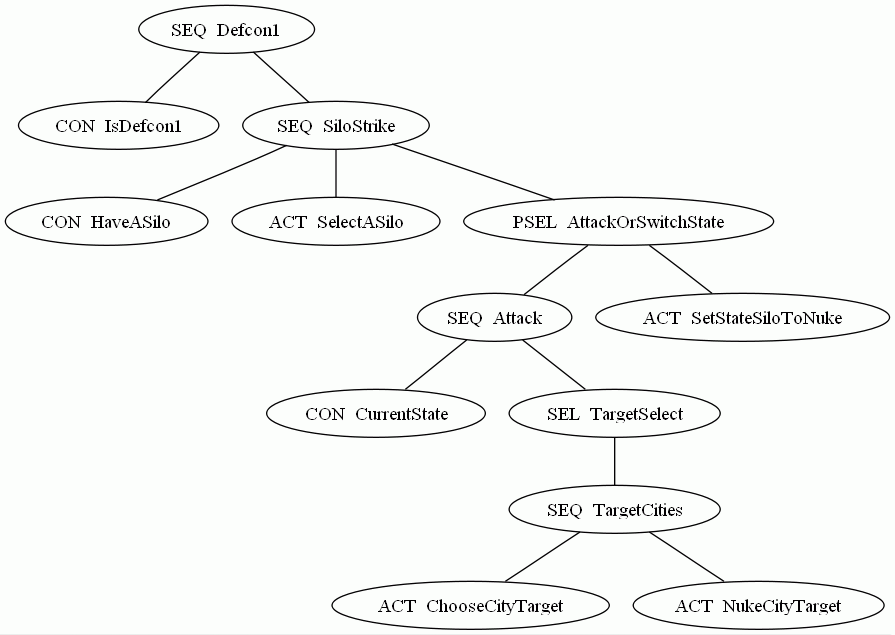
\includegraphics[scale=0.4]{images/defcon1r.png}
        \caption{Defcon 1}        
        \end{center} 
    \end{figure}
